\documentclass[openright,twoside]{iitbthesis}
\usepackage{graphicx} % Required for inserting images
\usepackage{epsfig} 
\usepackage{amsmath} 
\usepackage{amssymb}  
\usepackage{circuitikz}
\usepackage{mathdots}
\usepackage[inline]{enumitem}                   
\usepackage{wrapfig}
\usepackage{booktabs}
\usepackage{multirow}
\usepackage{scalefnt}
\usepackage{multicol}
\usepackage{bm}
\usepackage{bbm}
\usepackage{dsfont}
\usepackage{nicematrix}
\usepackage{verbatim}
\usepackage{mathrsfs}
\usepackage{mathtools}
\usepackage{commands}
\usepackage{theorems}
\usepackage{environments}
\usepackage{longtable}
\usepackage{microtype}
\usepackage{tabularx}
\usepackage{array}
\usepackage{ragged2e}
\setlength{\emergencystretch}{2em}
%Tikz Settings for figures
\usepackage{tikz-cd}
\usepackage{tikz}
\usepackage{subcaption}
%\usepackage{subfigure}
\usetikzlibrary{arrows, matrix}
\usetikzlibrary{arrows.meta, angles, quotes, calc}
\usetikzlibrary{shapes, arrows, calc, arrows.meta, fit, positioning}%graphs,graphdrawing} %\usegdlibrary{layered}
\tikzset{  
-Latex,auto,node distance =2 cm and 1.3 cm, thick,% node distance is the distance between one node to other, where 1.5cm is the length of the edge between the nodes  
state/.style ={circle, draw, minimum width = 0.9 cm}, % the minimum width is the width of the ellipse, which is the size of the shape of vertex in the node graph  
point/.style = {circle, draw, inner sep=0.18cm, fill, node contents={}},  
dotteddirected/.style={-Latex,loosely dash dot}, % it is the edge having two directions  
reverseedge/.style={-Latex,dotted}, % it is the dashed directed edge
el/.style = {inner sep=2.5pt, align=right, sloped}  
}
\title{Analysis \& Synthesis of Networked Dynamical Systems: Stability, Performance and Applications of Consensus}
\author{Avinash Kumar Dubey}
\date{\today}
\rollnum{184076010}
%\iitbdegree{Doctor of Philosophy}
\reporttype{Synopsis}
\department{DEPARTMENT OF ELECTRICAL ENGINEERING}
\setguide{Prof. Dwaipayan Mukherjee}


\makeatletter
\renewcommand{\maketitle}{%
  \begin{titlepage}
    \let\footnotesize\small \let\footnoterule\relax \setcounter{page}{1}
    \vspace*{0.1in}
    \begin{center}
      \mbox{}\\
      % 1. Print Thesis Title in Uppercase
      {\bf\expandafter\uppercase\expandafter{\LARGE\@title}} \\[\@thesistitlebigskip]
      
      % 2. Print "SYNOPSIS" instead of "Submitted in partial fulfillment..."
      {\LARGE \bf Synopsis} \\[\@thesistitlebigskip]
      
      {\large by} \\[\@thesistitlemedskip]
      {\large \bf \@author} \\
      {\large \bf (Roll No. \@rollnum)} \\[\@thesistitlebigskip]
      {\large Supervisor: }  \\
      {\large \bf \@advisorname} \\
      \ifx\@coadvisorname\@empty
         \ifx\@exadvisorname\@empty
             \mbox{}\\[\@thesistitlebigskip]
         \else
             {\large and } \\
             {\large \bf \@exadvisorname} \\[\@thesistitlemedskip]
         \fi
      \else
          \ifx\@exadvisorname\@empty
              {\large and } \\
              {\large \bf \@coadvisorname} \\[\@thesistitlemedskip]
          \else
              {\large \bf \@coadvisorname} \\
              {\large and } \\
              {\large \bf \@exadvisorname} \\[\@thesistitlemedskip]
          \fi
      \fi
      \begin{center}
      
\includegraphics[scale=0.21]{iit_logo2.jpg}
      \end{center}
      {\large \uppercase{\@department}} \\
      {\large INDIAN INSTITUTE OF TECHNOLOGY BOMBAY}\\%
      {\large \@date}
    \end{center}
  \end{titlepage}
  \setcounter{footnote}{0}
  \setcounter{page}{1}
}
\makeatother


\begin{document}
\maketitle
\begin{abstract}
This thesis investigates consensus in networked dynamical systems with a primary emphasis on the structural influence of directed cycles on system stability, performance bounds, and subsequent trajectory synthesis. Networked multi-agent systems operating over topologies with directed feedback structures exhibit complex dynamical behaviors that frequently defy classical graph-theoretic consensus guarantees. For agents modelled as single-integrators, the introduction of reverse edges, leading to directed cycle formation, degrades the convergence rate to consensus when a directed spanning tree already exists. In contrast, for second-order agent dynamics, the presence of directed cycles can induce severe structural instabilities, leading to a complete breakdown of consensus despite the presence of a spanning tree. This instability originates from the stringent lower bound required on the velocity coupling gain, denoted by $\gamma$, which is introduced by reverse-edge feedback channels.

Existing polynomial-based Laplacian spectral analysis techniques enable the estimation of admissible bounds on this coupling gain $\gamma$ without explicitly computing the exact graph Laplacian spectrum; however, these analytical methods are restricted to configurations where the root or leader node remains strictly outside the directed cycle formed by the additional reverse edges. When the leader node itself participates in the directed cycle formation, traditional polynomial approaches fail entirely in providing reliable stability margins. This is because such a scenario causes a fundamental structural collapse in the graph hierarchy, effectively converting all nodes within the cycle consisting the root into co-equal/equivalent root nodes-- a situation that has historically remained unaddressed in the literature. To address this issue, this thesis first investigates the interplay of multiple directed loops, specifically analyzing how the addition of a secondary directed cycle modifies the mathematical bounds on the velocity coupling factor. Building upon these bounds, we propose a novel, decentralized edge perturbation method targeted directly at the edges within and immediately surrounding the directed loops. This edge perturbation strategy guarantees consensus for any pre-designed coupling gain $\gamma$. The key advantage of this framework is twofold: first, the required perturbations are strictly localized to the loop structure, ensuring no interference with the remainder of the network, or requirement of any global parameter tuning by any of the agent. Second, by utilizing a root-locus-based analytical framework, the methodology ensures stability guarantees even when the leader node actively participates in the loop structure.

Moving beyond stability, the thesis extends into performance optimization by examining the structural role of cycles in networks of double-integrators from an $\mathcal{H}_2$ norm perspective. While cycles are well known to alter the algebraic connectivity (Fiedler eigenvalue) and convergence rate, their precise impact on systemic performance metrics such as disturbance attenuation remains under-explored. Using an undirected path graph as the nominal spanning tree, we systematically evaluate the $\mathcal{H}_2$ performance of networks containing up to two cycles. It is formally demonstrated that $\mathcal{H}_2$ performance fundamentally depends on the underlying spanning tree topology, the spatial length of the cycles, their relative overlap, and, crucially, their absolute spatial placement relative to the root node. In particular, our performance analysis reveals that longer cycles exhibiting partial structural overlap can yield significantly improved $\mathcal{H}_2$ disturbance rejection compared to non-overlapping loop configurations. We characterize the extent of overlap that optimizes performance, thereby providing explicit structural guidelines for designing robust network architectures for agents modelled as double integrators.

Finally, applying the idea of consensus to the domain of cooperative interception problems, the thesis presents a dual-stage trajectory planning framework for autonomous agents, subject to non-holonomic constraints, lateral acceleration bounds, and strict terminal impact-angle and impact-time constraints. We first develop a Dubins-type path planning strategy that satisfies simultaneous space-time impact requirements by systematically modulating the radius of a virtual circle. The admissible bounds of this designed radius is analytically characterized as a function of the initial engagement geometry, providing simulation-backed design guarantees for unique path synthesis. The Dubins-type guidance law requires only piecewise-constant lateral acceleration over distinct engagement phases, rendering it highly attractive for implementation. To address the physical rigidity and curvature discontinuities inherent in fixed-radius Dubins-type paths, we introduce an Archimedean spiral-based path planning methodology. By exploiting the additional degree of freedom inherent in Archimedean spirals through an additional parameter, this strategy enables continuous curvature variation, substantially enlarging the feasible solution space, and also improving robustness under tight lateral acceleration bounds.The synthesis is ultimately extended to multi-agent interception scenarios by coupling the spiral trajectory generator with decentralized consensus protocols. The resulting unified framework leverages the idea of consensus and cooperative guidance design, thereby providing both stability guarantees and practical trajectory synthesis algorithms for coordinated autonomous operations.
\end{abstract}
%\chapter{Synopsis}
{\Huge \textbf{SYNOPSIS}}
\section{Consensus Breakdown and Bound on Velocity Coupling Factor $\gamma$: }
%\noindent \textbf{Section 1: Consensus Breakdown and Bound on Velocity Coupling Factor $\gamma$: }

Building upon early work on single-integrators over undirected topologies, Ren and Atkins, extended consensus protocols to double-integrator agent dynamics over directed network topologies. Consider $N$ double-integrator agents operating under the distributed control law:
\begin{equation} \label{eq:agent-wise}
	u_i(t) = -\sum_{j=1}^{N} w_{ij} \left[ (p_i(t) - p_j(t)) + \gamma (v_i(t) - v_j(t)) \right], \quad i \in \{1, 2, \dots, N\}
\end{equation}
where $p_i(t), v_i(t) \in \mathbb{R}^d$ represent the position and velocity vectors of agent $i$, $w_{ij}$ is the $(i,j)$-th entry of the weighted adjacency matrix $\mathcal{W}$, and $\gamma > 0$ is the \textbf{velocity coupling parameter}.

It was observed that while protocol \eqref{eq:agent-wise} seamlessly achieves consensus over acyclic topologies, consensus can suddenly break down when directed cycles are present in the network graph. To guarantee consensus over general digraphs containing a directed spanning tree, Ren and Atkins established a conservative sufficient lower bound on the velocity coupling parameter $\gamma$:

\begin{equation}\label{eq:ren_gamma_bound}
    \gamma > \max_{i \in \{2, \dots, N\}} \sqrt{\frac{2}{\mathfrak{Re}(\lambda_i)}}
\end{equation}
where $\lambda_i$ denotes the $i$-th non-zero eigenvalue of the graph Laplacian matrix $\mathcal{L}$, ordered by real parts such that $0 = \lambda_1 < \mathfrak{Re}(\lambda_2) \le \dots \le \mathfrak{Re}(\lambda_N)$.

\begin{figure}[ht!]
    \centering
    \begin{subfigure}[b]{0.45\textwidth}
        \centering
        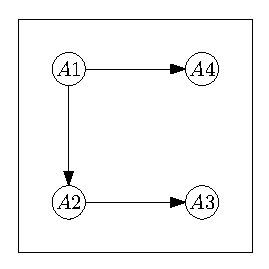
\includegraphics[scale=1]{Sapnning.eps}
        \caption{Consensus achieved for $\gamma = 0.1$ over an acyclic directed spanning tree topology.}
        \label{fig:spanning_tree_consensus}
    \end{subfigure}
    \hfill
    \begin{subfigure}[b]{0.45\textwidth}
        \centering
        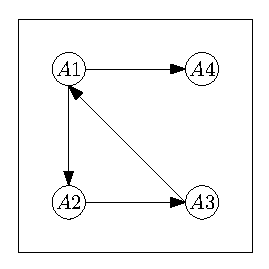
\includegraphics[scale=1]{Cycle.eps}
        \caption{Breakdown of consensus due to the presence of directed cycles.}
        \label{fig:cycle_consensus_failure}
    \end{subfigure}
    \caption{Comparison of double-integrator consensus behavior over acyclic vs. cyclic directed topologies.}
    \label{fig:topological_consensus_comparison}
\end{figure}


Subsequently, Yu et al. derived the exact necessary and sufficient condition for second-order consensus over directed topologies. Specifically, the velocity coupling factor $\gamma$ must satisfy:
\begin{equation}\label{eq:yu_gamma_exact_bound}
    \gamma > \max_{i \in \{2, \dots, N\}} \frac{|\mathfrak{Im}(\lambda_i)|}{|\lambda_i|} \sqrt{\frac{1}{\mathfrak{Re}(\lambda_i)}}
\end{equation}
where $|\lambda_i| = \sqrt{\mathfrak{Re}(\lambda_i)^2 + \mathfrak{Im}(\lambda_i)^2}$ is the magnitude of the $i$-th Laplacian eigenvalue.

In acyclic networks (such as directed chains or trees), all non-zero Laplacian eigenvalues are purely real ($\mathfrak{Im}(\lambda_i) = 0$), reducing the right-hand side of \eqref{eq:yu_gamma_exact_bound} to zero and permitting consensus for any arbitrarily small choice of $\gamma > 0$. However, when directed cycles exist, complex-conjugate eigenvalue pairs emerge with non-zero imaginary parts ($\mathfrak{Im}(\lambda_i) \neq 0$), imposing a strictly positive lower bound on $\gamma$. 

If an operational network has a fixed, predesigned velocity coupling factor $\gamma$, the introduction of reverse feedback channels shifts the Laplacian spectrum outward in the complex plane, potentially violating condition \eqref{eq:yu_gamma_exact_bound} and triggering system instability.

This vulnerability under cyclic topologies motivates the core research problem addressed in this section.
\begin{problem}\label{prob:multi_loop_coupling}
    Analyze how the presence of multiple interacting directed loops (whether disjoint, overlapping, or sharing root/leader nodes) modifies the analytical bounds on the velocity coupling parameter $\gamma$ across chain topologies, and formulate local edge/node perturbation methodologies to guarantee consensus under fixed coupling constraints.
\end{problem}
\noindent \textbf{Solution \ref{prob:multi_loop_coupling}}

Consider a nominal $N$-node directed chain with unit forward edge weights ($w_{i+1, i} = 1$ for all $i \in \{1, \dots, N-1\}$). To introduce feedback mechanisms, we augment the chain with two reverse edges:
\begin{itemize}
    \item \textbf{Reverse Edge 1:} Originates at tail node $y_1$ and terminates at head node $x_1$ ($y_1 > x_1$), forming Cycle~1 of length $\ell_1 \coloneqq y_1 - x_1$.
    \item \textbf{Reverse Edge 2:} Originates at tail node $y_2$ and terminates at head node $x_2$ ($y_2 > x_2$), forming Cycle~2 of length $\ell_2 \coloneqq y_2 - x_2$.
\end{itemize}

\begin{remark}\label{rem:ch_TRE_cyclelengthdef}
Following graph-theoretic conventions for chain topologies, the cycle length $\ell \coloneqq y - x$ denotes one less than the cardinality of vertices participating in the directed cycle.
\end{remark}

Without loss of generality, we order the head nodes such that $x_1 \le x_2$. Based on the relative spatial orientation and intersection of these two reverse edges, there exist six exhaustive, mutually exclusive topological configurations, illustrated in Figures~\ref{fig:cases_all}(a)--\ref{fig:cases_all}(f):

\begin{enumerate}
    \item \textbf{Case 1 (Completely Disjoint Cycles):} $x_1 < y_1 < x_2 < y_2$. The two cycles share no common nodes or edges ($\mathcal{V}_1 \cap \mathcal{V}_2 = \emptyset$), as shown in Figure~\ref{fig:case1}.
    \item \textbf{Case 2 (Edge-Disjoint Cycles with a Shared Node):} $x_1 < y_1 = x_2 < y_2$. The tail of Reverse Edge~1 coincides with the head of Reverse Edge~2 ($\mathcal{V}_1 \cap \mathcal{V}_2 = \{y_1\}$), as shown in Figure~\ref{fig:case2}.
    \item \textbf{Case 3 (Partially Overlapping Cycles):} $x_1 < x_2 < y_1 < y_2$. The cycles overlap along an intermediate sub-chain, but neither is strictly nested within the other, as shown in Figure~\ref{fig:case3}.
    \item \textbf{Case 4 (Fully Nested Cycles with Disjoint Endpoints):} $x_1 < x_2 < y_2 < y_1$. Cycle~2 is strictly contained within Cycle~1 ($\mathcal{V}_2 \subset \mathcal{V}_1$), with both endpoints disjoint, as shown in Figure~\ref{fig:case4}.
    \item \textbf{Case 5 (Fully Nested Cycles with a Shared Tail Node):} $x_1 < x_2 < y_1 = y_2$. Cycle~2 is nested within Cycle~1, with both feedback edges originating from the same tail node, as shown in Figure~\ref{fig:case5}.
    \item \textbf{Case 6 (Fully Nested Cycles with a Shared Head Node):} $x_1 = x_2 < y_2 < y_1$. Cycle~2 is nested within Cycle~1, with both feedback edges terminating at the same head node, as shown in Figure~\ref{fig:case6}.
\end{enumerate}

Each of Cases~1--3 further bifurcates into three length-dependent regimes: (a)~$\ell_1 > \ell_2$, (b)~$\ell_2 > \ell_1$, and (c)~$\ell_1 = \ell_2$. 
\begin{theo}[Spectral Boundary for Case 1 Topologies]\label{Theoremcase1}
Consider an $N$-node directed chain with unit forward edge weights containing two completely disjoint reverse edges under \textbf{Case 1} ($x_1 < y_1 < x_2 < y_2$). The dominant Laplacian convergence root $\lambda_2 = 1 - s_1$ is determined by the unique real solution $s_1 \in (0,1)$ of:
\begin{equation}\label{eq:case1_theorem_statement}
	\begin{cases}
		s^{\ell_1+1} + s^{\ell_1} - 1 = 0, & \text{if } \ell_1 > \ell_2 \\
		s^{\ell_2+1} + s^{\ell_2} - 1 = 0, & \text{if } \ell_2 > \ell_1 \\
		s^{\ell_1+1} + s^{\ell_1} - 1 = 0, & \text{if } \ell_1 = \ell_2
	\end{cases}
\end{equation}
\end{theo}
\begin{theo}[Spectral Boundary for Case 2 Topologies]\label{Theoremcase2}
Consider an $N$-node directed chain with unit forward edge weights containing two reverse edges under \textbf{Case 2} ($y_1 = x_2$). The dominant Laplacian convergence root $\lambda_2 = 1 - s_1$ is determined by the unique real root $s_1 \in (0,1)$ of:
\begin{equation}\label{eq:case2_theorem_statement}
	\begin{cases}
		s^{\ell_1+1} + 2s^{\ell_1} + s^{\ell_1-1} - s^{\ell_1-\ell_2} - s^{\ell_1-\ell_2-1} = 1, & \text{if } \ell_1 > \ell_2 \\
		s^{\ell_2+2} + 2s^{\ell_2+1} + s^{\ell_2} - s^{\ell_2-\ell_1+1} - s = 1, & \text{if } \ell_2 > \ell_1 \\
		s^{\ell_2+2} + 2s^{\ell_2+1} + s^{\ell_2} - 2s = 1, & \text{if } \ell_1 = \ell_2
	\end{cases}
\end{equation}
\end{theo}
\begin{theo}[Spectral Boundary for Case 3 Topologies]\label{theo9}
Consider an $N$-node directed chain under \textbf{Case 3} (partially overlapping cycles, $x_1 < x_2 < y_1 < y_2$). The dominant Laplacian convergence root $\lambda_2 = 1 - s_1$ is determined by the unique real solution $s_1 \in (0,1)$ of:
\begin{equation}
	\begin{cases}
		s^{\ell_1+1} + 2s^{\ell_1} + s^{\ell_1-1} - s^{\ell_1-\ell_2} - s^{\ell_1-\ell_2-1} = 1, & \text{if } \ell_1 > \ell_2 \\
		s^{\ell_2+2} + 2s^{\ell_2+1} + s^{\ell_2} - s^{\ell_2-\ell_1+1} - s = 1, & \text{if } \ell_2 > \ell_1 \\
		s^{\ell_2+2} + 2s^{\ell_2+1} + s^{\ell_2} - 2s = 1, & \text{if } \ell_1 = \ell_2
	\end{cases}
\end{equation}
\end{theo}
\begin{theo}[Spectral Boundary for Case 4 Topologies]\label{Theoremcase4}
Consider an $N$-node directed chain with unit forward edge weights containing two fully nested reverse edges under \textbf{Case 4} ($x_1 < x_2 < y_2 < y_1$, with $\ell_1 > \ell_2$). The dominant Laplacian convergence root $\lambda_2 = 1 - s_1$ is determined by the unique real solution $s_1 \in (0,1)$ of
\begin{equation}\label{eq:case4_theorem_statement}
	s^{\ell_1+1} + 2s^{\ell_1} + s^{\ell_1-1} - s^{\ell_1-\ell_2} - s^{\ell_1-\ell_2-1} = 1.
\end{equation}
\end{theo}
\begin{theo}[Spectral Boundary for Case 5 Topologies]\label{Theoremcase5}
Consider an $N$-node directed chain under \textbf{Case 5} (nested cycles sharing tail node $y_1 = y_2$, with $\ell_1 > \ell_2$). The dominant Laplacian convergence root $\lambda_2 = 1 - s_1$ is determined by the unique real solution $s_1 \in (0,1)$ of:
\begin{equation}\label{eq:case5_theorem_statement}
	s^{\ell_1+1} + 2s^{\ell_1} + s^{\ell_1-1} - s^{\ell_1-\ell_2} - s^{\ell_1-\ell_2-1} = 1
\end{equation}
\end{theo}
\begin{theo}[Spectral Boundary for Case 6 Topologies]\label{theo10}
Consider an $N$-node directed chain under \textbf{Case 6} (nested cycles sharing head node $x_1 = x_2$, with $\ell_1 > \ell_2$). The dominant Laplacian convergence root $\lambda_2 = 1 - s_1$ is determined by the unique real solution $s_1 \in (0,1)$ of:
\begin{equation}\label{eq:case6_statement}
	s^{\ell_1}(s+2) - s^{\ell_1-\ell_2} = 1
\end{equation}
\end{theo}


\begin{figure}[htbp]
    \centering
    % --- Row 1 ---
    \begin{subfigure}[b]{0.48\textwidth}
        \centering
        \resizebox{\linewidth}{!}{%
        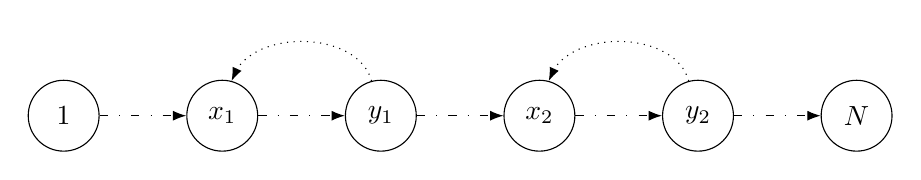
\begin{tikzpicture}[node distance=1.1cm]
            \node[state] (root) {$1$};
            \node[state, right=of root] (x1) {$x_1$};
            \node[state, right=of x1] (y1) {$y_1$};
            \node[state, right=of y1] (x2) {$x_2$};
            \node[state, right=of x2] (y2) {$y_2$};
            \node[state, right=of y2] (N) {$N$};
            \path [dotteddirected] (root) edge (x1);
            \path [dotteddirected] (x1) edge (y1);
            \path [dotteddirected] (y1) edge (x2);
            \path [dotteddirected] (x2) edge (y2);
            \path [dotteddirected] (y2) edge (N);
            \path [reverseedge] (y1) edge[bend right=75] (x1);
            \path [reverseedge] (y2) edge[bend right=75] (x2);
        \end{tikzpicture}%
        }
        \caption{Completely disjoint cycles}
        \label{fig:case1}
    \end{subfigure}\hfill
    \begin{subfigure}[b]{0.48\textwidth}
        \centering
        \resizebox{\linewidth}{!}{%
        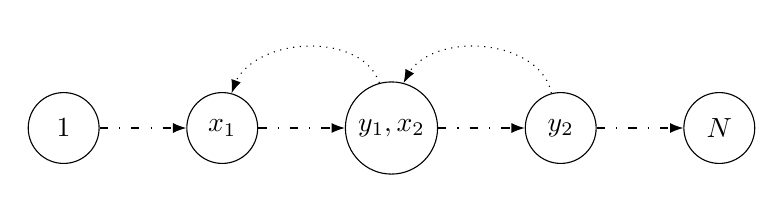
\begin{tikzpicture}[node distance=1.1cm]
            \node[state] (root) {$1$};
            \node[state, right=of root] (x1) {$x_1$};
            \node[state, right=of x1] (y1) {$y_1, x_2$};
            \node[state, right=of y1] (y2) {$y_2$};
            \node[state, right=of y2] (N) {$N$};
            \path [dotteddirected] (root) edge (x1);
            \path [dotteddirected] (x1) edge (y1);
            \path [dotteddirected] (y1) edge (y2);
            \path [dotteddirected] (y2) edge (N);
            \path [reverseedge] (y1) edge[bend right=75] (x1);
            \path [reverseedge] (y2) edge[bend right=75] (y1);
        \end{tikzpicture}%
        }
        \caption{Edge-disjoint cycles sharing a node}
        \label{fig:case2}
    \end{subfigure}

    \vspace{0.4cm}

    % --- Row 2 ---
    \begin{subfigure}[b]{0.48\textwidth}
        \centering
        \resizebox{\linewidth}{!}{%
        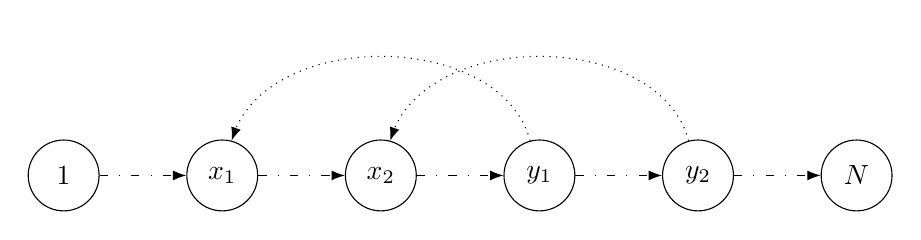
\begin{tikzpicture}[node distance=1.1cm]
            \node[state] (root) {$1$};
            \node[state, right=of root] (x1) {$x_1$};
            \node[state, right=of x1] (x2) {$x_2$};
            \node[state, right=of x2] (y1) {$y_1$};
            \node[state, right=of y1] (y2) {$y_2$};
            \node[state, right=of y2] (N) {$N$};
            \path [dotteddirected] (root) edge (x1);
            \path [dotteddirected] (x1) edge (x2);
            \path [dotteddirected] (x2) edge (y1);
            \path [dotteddirected] (y1) edge (y2);
            \path [dotteddirected] (y2) edge (N);
            \path [reverseedge] (y1) edge[bend right=75] (x1);
            \path [reverseedge] (y2) edge[bend right=75] (x2);
        \end{tikzpicture}%
        }
        \caption{Partially overlapping cycles}
        \label{fig:case3}
    \end{subfigure}\hfill
    \begin{subfigure}[b]{0.48\textwidth}
        \centering
        \resizebox{\linewidth}{!}{%
        \begin{tikzpicture}[node distance=1.1cm]
            \node[state] (root) {$1$};
            \node[state, right=of root] (x1) {$x_1$};
            \node[state, right=of x1] (x2) {$x_2$};
            \node[state, right=of x2] (y2) {$y_2$};
            \node[state, right=of y2] (y1) {$y_1$};
            \node[state, right=of y1] (N) {$N$};
            \path [dotteddirected] (root) edge (x1);
            \path [dotteddirected] (x1) edge (x2);
            \path [dotteddirected] (x2) edge (y2);
            \path [dotteddirected] (y2) edge (y1);
            \path [dotteddirected] (y1) edge (N);
            \path [reverseedge] (y1) edge[bend right=85] (x1);
            \path [reverseedge] (y2) edge[bend right=65] (x2);
        \end{tikzpicture}%
        }
        \caption{Fully nested cycles (disjoint reverse edges)}
        \label{fig:case4}
    \end{subfigure}

    \vspace{0.4cm}

    % --- Row 3 ---
    \begin{subfigure}[b]{0.48\textwidth}
        \centering
        \resizebox{\linewidth}{!}{%
        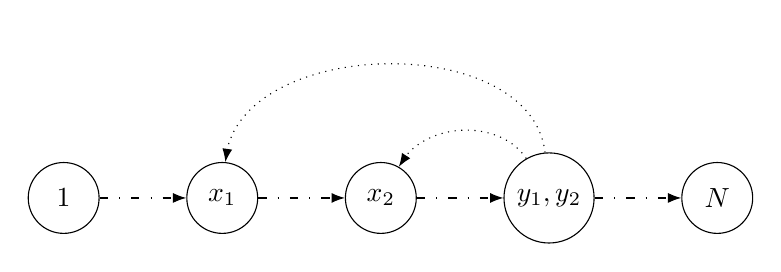
\begin{tikzpicture}[node distance=1.1cm]
            \node[state] (root) {$1$};
            \node[state, right=of root] (x1) {$x_1$};
            \node[state, right=of x1] (x2) {$x_2$};
            \node[state, right=of x2] (y1) {$y_1, y_2$};
            \node[state, right=of y1] (N) {$N$};
            \path [dotteddirected] (root) edge (x1);
            \path [dotteddirected] (x1) edge (x2);
            \path [dotteddirected] (x2) edge (y1);
            \path [dotteddirected] (y1) edge (N);
            \path [reverseedge] (y1) edge[bend right=85] (x1);
            \path [reverseedge] (y1) edge[bend right=60] (x2);
        \end{tikzpicture}%
        }
        \caption{Fully nested cycles sharing a tail node}
        \label{fig:case5}
    \end{subfigure}\hfill
    \begin{subfigure}[b]{0.48\textwidth}
        \centering
        \resizebox{\linewidth}{!}{%
        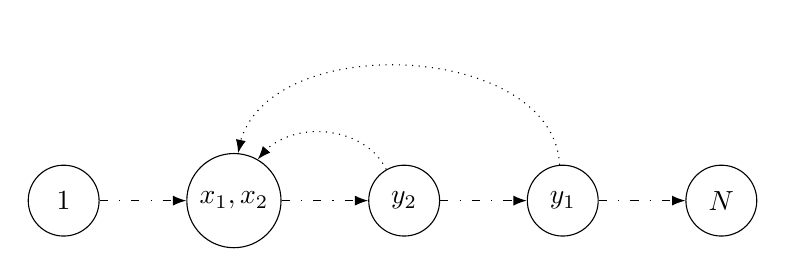
\begin{tikzpicture}[node distance=1.1cm]
            \node[state] (root) {$1$};
            \node[state, right=of root] (x1) {$x_1, x_2$};
            \node[state, right=of x1] (y2) {$y_2$};
            \node[state, right=of y2] (y1) {$y_1$};
            \node[state, right=of y1] (N) {$N$};
            \path [dotteddirected] (root) edge (x1);
            \path [dotteddirected] (x1) edge (y2);
            \path [dotteddirected] (y2) edge (y1);
            \path [dotteddirected] (y1) edge (N);
            \path [reverseedge] (y1) edge[bend right=85] (x1);
            \path [reverseedge] (y2) edge[bend right=60] (x1);
        \end{tikzpicture}%
        }
        \caption{Fully nested cycles sharing a head node}
        \label{fig:case6}
    \end{subfigure}

    \caption{The six mutually exclusive topological configurations arising from two reverse feedback edges added to an $N$-node directed chain.}
    \label{fig:cases_all}
\end{figure}
\section{The Root-Node Loop Structural Singularity}
Standard polynomial-based spectral analysis techniques (such as Routh-Hurwitz criteria on Laplacian characteristic equations) rely on the root node (leader) having an in-degree of zero ($d_{in,1} = 0$). Under this condition, the root node acts as an autonomous leader unaffected by downstream feedback.

However, when a reverse communication edge enters the root node itself ($x_1 = 1$), such a hierarchical structure, which preserves the root node, collapses. The root node loses its hierarchical immunity ($d_{in,1} > 0$), and \textbf{every node within the directed cycle effectively becomes an equivalent root node}.
\begin{problem}\label{prob:root_node_singularity}
    When the leader/root participates in a loop, standard characteristic polynomials yield trivial solutions ($s_1 = 1$), failing to provide reliable stability bounds. The literature lacks a fully decentralized framework capable of guaranteeing consensus when the root node is embedded in a loop, without requiring agents to access global spectrum knowledge or retune the global parameter $\gamma$. Address this issue by possibly designing a local gain-tuning strategy in the face of such a loop-formation.
\end{problem}
\noindent \textbf{Solution \ref{prob:root_node_singularity}}

We synthesized a suite of \textbf{fully localized control remedies} that guarantee second-order consensus under fixed global coupling parameters $\gamma$. 
\begin{enumerate}
    \item \textbf{Decentralized Gershgorin--Based Perturbation Framework (Leader -- Exterior Loops):} For directed cycles that do not contain the leader/root node, we formulate \textbf{Node-Scaling, Edge-Scaling, and Combined-Scaling} algorithms. By constructing optimal Arithmetic Progressions (AP) of Gershgorin column discs, we guarantee that the minimum real eigenvalue component satisfies $\mathfrak{Re}(\lambda_2) \ge 1/\gamma^2$, ensuring consensus through localized gains confined strictly to loop agents and edges.
    \item \textbf{Resolution of the Root-Node Loop Singularity via Complementary Root-Locus:} For directed cycles that incorporate the leader node, where Gershgorin-based methods fail, we formulate a complementary root-locus control framework. By modeling loop gain shifts via $G(s) = \frac{\beta\{(s-\alpha)^\ell - (-\alpha)^\ell\}}{s(s-\alpha)^\ell}$, we derive precise gain bounds on $\alpha$ and $\beta$ that guarantee stability.
    \item \textbf{Equal-Weight Cyclic Pursuit Synthesis:} To prevent edge-weakening under root-node loops, we derive an exact closed-form single-gain threshold ($\alpha \ge \frac{\cot^2(\pi/(\ell+1))}{2\gamma^2}$) based on cyclic pursuit, guaranteeing consensus while maintaining equal edge weights across all agents in the directed cycle.
\end{enumerate}
\begin{theo}[Node-Based Scaling Consensus Guarantee]\label{theo1}
Consider an $N$-node directed chain of double-integrator agents operating under protocol \eqref{eq:ch_GC_control_law} with fixed coupling $\gamma > 0$. Suppose a reverse edge of unit weight ($w_r = 1$) is inserted from node $y_1$ to node $x_1$ ($x_1 > 1$, range $\ell = y_1 - x_1$). Second-order consensus is guaranteed if the control law $u_i(t)$ of each node $i \in \{x_1, x_1+1, \dots, y_1\}$ is scaled by local factor $p_{i-x_1+1} > 0$:
\begin{equation}\label{eq:ch_GC_NodeScalar_formula}
	p_{i-x_1+1} = \left( \frac{\ell+1}{\gamma^2} + \epsilon \right) + (i - x_1) \frac{\frac{\ell+1}{\gamma^2} + \epsilon}{\ell + 1}, \quad \text{for any } \epsilon > 0
\end{equation}
\end{theo}
\begin{theo}[Edge-Based Scaling Consensus Guarantee]\label{theo2}
Consider an $N$-node directed chain of double integrators operating under protocol \eqref{eq:ch_GC_control_law} with fixed coupling $\gamma > 0$. Suppose a reverse edge of weight $w_r > 0$ is added from $y_1$ to $x_1$ ($x_1 > 1$, range $\ell$). Second-order consensus is guaranteed if forward edge weights $\{w_1, w_2, \dots, w_{\ell+1}\}$ are tuned as:
\begin{equation}\label{eq:ch_GC_ESScalar_formula}
	w_1 = \frac{\ell+1}{\gamma^2} + \epsilon, \quad w_k = w_1 + (k-1) \frac{w_1}{\ell+1}, \quad \text{for any } \epsilon > 0, k \in \{2, \dots, \ell+1\}
\end{equation}
\end{theo}
\begin{theo}[Root-Locus Gain Scaling Consensus Guarantee]\label{theo3ES}
\leavevmode\par\noindent
Consider an $N$-node directed chain of double integrators operating under protocol \eqref{eq:ch_GC_control_law} with fixed coupling $\gamma > 0$. Suppose a reverse edge is added from $y_1$ to $x_1 = 1$ ($x_1 = 1$, range $\ell$). Select node scaling factor $\alpha > 1/\gamma^2$. Then, there exists a upper gain bound $\bar{\beta} > 0$ such that when the control law of one agent in the loop is scaled by $\beta / \alpha$ (with $0 < \beta < \bar{\beta}$), second-order consensus is guaranteed.
\end{theo}
\section{$\mathcal{H}_2$ Performance and Disturbance Attenuation in Cyclic Topologies}
Beyond deterministic convergence, real-world multi-agent networks operate under environmental disturbances and sensor noise. The $\mathcal{H}_2$ norm measures total transient energy and stochastic noise amplification from exogenous inputs to network state deviations.

In single-integrator networks, it is known that the $\mathcal{H}_2$ performance is invariant to the choice of spanning tree and cycle location. For double-integrator networks, however, state dynamics are coupled through position and velocity integrators and such relationships or lack thereof between the performance and the choice of some specific spanning trees is largely unexplored.

\begin{problem}\label{prob:H2_Analysis}
    Derive, if possible, closed-form expressions for the $\mathcal{H}_2$ norm in a network of consensus-seeking double-integrators over path graphs. Quantify how cycle length, spatial placement of cycles relative to the root node, and partial structural overlap between two cycles dictate the overall $\mathcal{H}_2$ performance. 
\end{problem}
\noindent \textbf{Solution \ref{prob:H2_Analysis}}
\begin{enumerate}
    \item \textbf{Exact Closed-Form $\mathcal{H}_2$ Norm Expression:} By constructing an edge-space projection $\Sigma_e$ that decouples the unobservable rigid-body drift modes, we derive the exact, closed-form solution to the 2x2 block Lyapunov equation, proving that a double-integrator network always exhibits a larger $\mathcal{H}_2$ norm (poorer noise attenuation) than a single-integrator network.
    \item \textbf{Spanning Tree and Spatial Locality Sensitivity:} Unlike single-integrator systems (where all spanning trees and cycle locations yield identical $\mathcal{H}_2$ performance), we prove that for double integrators, the $\mathcal{H}_2$ norm does depend on the choice of spanning tree and the spatial location of the cycle. Specifically, placing a cycle near the spatial center of a path graph reduces the system's $\mathcal{H}_2$ norm.
    \item \textbf{Optimal Two-Cycle Overlap Bound:} For networks containing two interacting cycles, we utilize Jensen's Inequality to prove that completely non-overlapping cycles are suboptimal. We derive exact analytical upper bounds on the extent of edge overlap $s \coloneqq  k_1 + k_2$ that guarantees optimal noise suppression.
\end{enumerate}
\begin{theo}[ $\mathcal{H}_2$ Norm for Network of Double-Integrators]\label{theoH2}
\leavevmode\par\noindent
Consider an undirected multi-agent network of double integrators governed by minimal edge system $\Sigma$. The $\mathcal{H}_2$ norm is given by the following expression:
\begin{equation}\label{total_norm}
	\|\Sigma\|_2^2 = \frac{1}{2\gamma} \text{trace}\left[ (I_{n-1} - A_3^{-1}) (\sigma_r^2 I_{n-1} - \sigma_q^2 A_3^{-1}) \letree \right].
\end{equation}
Expanding \eqref{total_norm} yields the explicit structural representation:
\begin{equation}\label{total_norm_expanded}
	\|\Sigma\|_2^2 = \frac{1}{2\gamma} \text{trace}\left[ \sigma_r^2 \letree + (\sigma_q^2 + \sigma_r^2) (RR^T)^{-1} + \sigma_q^2 \left( (RR^T)^{-1} \letree^{-1} (RR^T)^{-1} \right) \right]
\end{equation}
\end{theo}
\begin{theo}[$\mathcal{H}_2$ Norm for Single-Cycle Path Graphs]\label{theo_single}
Let $\mathcal{P}_n$ be an $n$-node undirected path graph of double integrators subject to process noise $q(t)$ (variance $\sigma_q^2$) and measurement noise $r(t)$ (variance $\sigma_r^2$). The addition of a single edge forming a cycle of length $\ell = n_e - n_s < n$ results in an $\mathcal{H}_2$ norm given by:
\begin{equation}\label{eq:ch_RA_single_cycle_norm}
	\begin{aligned}
		\|\Sigma\|_2^2 = \frac{1}{2\gamma} &\left[ 2\sigma_r^2(n-1) + (\sigma_q^2 + \sigma_r^2)\left(n - 2 + \frac{1}{\ell+1}\right)  \right. \\
		&\quad \left. + \sigma_q^2 \frac{(n-1)(n+1)}{6} - \frac{\sigma_q^2(\ell+2)}{(\ell+1)^2} \text{trace}\left( T T^T \letree^{-1} \right) \right].
	\end{aligned}
\end{equation}

\end{theo}
\begin{theo}[Optimal Spatial Placement of a Single Cycle]\label{thm:ch_RA_single_cycle_location}
For a fixed cycle length $\ell = n_e - n_s$, the systemic $\mathcal{H}_2$ norm $\|\Sigma\|_2^2$ of a path graph $\mathcal{P}_n$ is strictly minimized when the cycle is positioned symmetrically at the spatial center of the network, corresponding to start node $n_s = \frac{n-\ell+1}{2}$ and center node $n_c = \frac{n+1}{2}$.
\end{theo}
\begin{theo}\label{overlap}
Consider an undirected path graph of double integrators on $n$ nodes ($n > 4$) containing two interacting cycles of lengths $\ell_1$ and $\ell_2$ sharing $s \ge 0$ tree edges resulting from the addition of two cycle-closing edges. Let $D(s)$ denote the performance scalar:
\begin{equation}\label{eq:ch_RA_Ds_def}
	D(s) \coloneqq \frac{\ell_1 + \ell_2 + 2}{(\ell_1+1)(\ell_2+1) - s^2}.
\end{equation}
Furthermore, let the baseline non-overlapping configuration ($s = 0$) span the total edge budget $\ell_1 + \ell_2 = n-1$ such that:
\begin{equation}\label{eq:ch_RA_baseline_lengths}
	(\ell_1, \ell_2) = \begin{cases} \left(\frac{n-1}{2}, \frac{n-1}{2}\right), & \text{for odd } n, \\[6pt] \left(\frac{n}{2}, \frac{n}{2}-1\right), & \text{for even } n, \end{cases}
\end{equation}
which achieves the baseline minimum scalar:
\begin{equation}
	D_{\min} \coloneqq \begin{cases} \frac{4}{n+1}, & \text{for odd } n, \\[6pt] \frac{4(n+1)}{n(n+2)}, & \text{for even } n. \end{cases}
\end{equation}
Then, there exists a non-trivial edge overlap $s > 0$ achieved by expanding the cycle lengths beyond their baseline values \eqref{eq:ch_RA_baseline_lengths} such that $D(s) \le D_{\min}$. Specifically, performance improvement ($D(s) \le D_{\min}$) is guaranteed whenever the spatial overlap increments $k_1$ and $k_2$ (where $s = k_1 + k_2$) satisfy:
\begin{enumerate}
	\item \textbf{For odd $n$:}
	\begin{equation}\label{odd_minD}
		\frac{k_1^2 + k_2^2 + k_1 k_2}{k_1 + k_2} \le \frac{n+1}{4}.
	\end{equation}
	\item \textbf{For even $n$:}
	\begin{equation}\label{even_minD}
		\frac{k_1^2 + k_2^2 + k_1 k_2}{k_1 + k_2} - \frac{k_2}{k_1 + k_2} \le \frac{n^2}{4(n+1)}.
	\end{equation}
\end{enumerate}
\end{theo}


\section{Trajectory Planning under Non-Holonomic and Spatio\-temporal Constraints}
Translating consensus principles to physical autonomous interceptors introduces kinematic and dynamic constraints. Classical Proportional Navigation Guidance (PNG) and Dubins curves suffer from major physical limitations:
\begin{itemize}
    \item Dubins Rigidity: Standard Dubins paths use fixed minimum turn radii ($r_m$), that do not offer any flexibility in the choice of \emph{impact time} or an interception mission's duration.
    \item Acceleration Bounds: Physical actuators saturate at $a^{\text{max}}$. If initial engagement geometry is unfavorable, standard guidance laws demand unachievable lateral acceleration ($a_M > a^{\text{max}}$), causing the interceptor to miss its target. 
\end{itemize}
\begin{problem}\label{prob:trajectory_plannning}
    Develop continuous-curvature, and acceleration-bounded guidance strategies that guarantee simultaneous satisfaction of spatial impact angle ($\zeta$) and temporal impact time ($t_{\text{imp}}$) constraints for single interceptors, and then extend such ideas to multi-interceptor teams by possibly exploiting the idea of consensus.
\end{problem}
\noindent \textbf{Solution \ref{prob:trajectory_plannning}}
An open-loop and equivalent closed-loop trajectory planning framework was synthesized using Dubins-like path geometry to achieve simultaneous terminal approach angle $\theta_t$ and terminal arrival time $t_{\text{imp}}$ constraints against stationary targets. This solution provided:
\begin{itemize}
    \item \textbf{Implementable Acceleration Profile:} The proposed guidance protocol demands piecewise-constant lateral acceleration across three discrete level acceleration profile ($+a^{\max}, 0, -a^{\max} \frac{r_m}{r_d}$), eliminating high-order polynomial computation and preventing actuator saturation.
    \item \textbf{Flexible Arrival Time Tuning:} Introducing variable secondary turn radius $r_d \ge r_m$ allows exact terminal time matching, while mirrored circle geometry ($C_2'$) renders achievable arrival times unbounded above.
    \item \textbf{Singularity-Free Closed-Loop Execution:} Distance-based closed-loop feedback \eqref{eq:ch_DP_closed_loop_guidance} with hyperbolic tangent smoothing removes trigonometric singularities at large lead angles ($\theta_M \approx 90^\circ$).
\end{itemize}
While Dubins trajectories provide a minimal-length piecewise-constant acceleration framework, their discrete curvature jumps ($\kappa \in \{+1/r_m, 0, -1/r_d\}$) introduce jump discontinuities in the lateral acceleration profile.To achieve continuous curvature trajectories without discontinuities in lateral acceleration, \textbf{spiral-based path geometries} present a powerful alternative. A two-phase adaptive guidance law and multi-agent coordination protocol was developed using generalized Archimedean spirals. 
\begin{enumerate}
    \item \textbf{Curvature Feasibility Analysis:} We derive exact closed-form expressions for the maximum curvature $\kappa_{\max} = f(\beta)/\alpha$ of generalized Archimedean spirals, establishing a sharp physical feasibility threshold $\alpha_{\text{ref}} \coloneqq v_p^2 f(\beta) / a_{\max}$.
    \item \textbf{Two-Phase Adaptive Scaling Control:} We formulate a two-phase guidance law that proactively adapts the scaling factor $\alpha(t) \to \alpha_{\text{ref}}$ during Phase 1 whenever $\alpha_0 < \alpha_{\text{ref}}$, eliminating lateral acceleration saturation before transitioning to Phase 2 terminal angle tracking.
    \item \textbf{Prescribed-Time Robust Error Suppression:} We integrate prescribed-time sliding mode control components into the adaptive spiral dynamics, proving finite-time error convergence $e(t) \to 0$ as $t \to T^*$ despite bounded process noise.
    \item \textbf{Directed Graph Multi-Agent Coordination:} We extend the single-agent framework to multi-agent swarms by executing directed chain consensus over the spiral parameter vector $\boldsymbol{\alpha}$, achieving synchronized, sector-allocated directional cooperative attacks across heterogeneous vehicle fleets.
\end{enumerate}

\section{Thesis Contributions and Novelty}
The primary analytical and application-oriented contributions of this thesis are summarized as follows:
\begin{itemize}
    \item \textbf{Dual-Loop Spectral Characterization in Directed Chains:} We establish exact univariate polynomial equations that dictate the dominant Laplacian convergence root $s_1 = 1 - \lambda_2$ across six distinct topological configurations of dual reverse edges. We prove that adding a cycle of length $l$ alters $l+1$ eigenvalues when the root node is excluded, but only $l$ eigenvalues when the root node is included.
    \item \textbf{Local Decentralized Perturbation Framework (Leader-Exterior Loops):} We introduce Gershgorin-disc-based Node Scaling, Edge Scaling, and Combined Scaling methods. By constructing Arithmetic Progressions (AP) of disc centers, these strategies guarantee second-order consensus for any predesigned coupling gain $\gamma$ through localized modifications confined strictly to loop edges and nodes.
    \item \textbf{Resolution of the Root-Node Loop Structural Singularity:} We provide the first framework in the literature to resolve consensus breakdown when the leader node is inside a feedback loop. Using a complementary root-locus formulation wherein a relevant transfer function of the form $G(s) = \frac{\beta_{RL}\{(s-\alpha_{RL})^l - (-\alpha_{RL})^l\}}{s(s-\alpha_{RL})^l}$ is used, we derive precise gain bounds that preserve stability. Furthermore, we prove that an equal-weight cyclic pursuit design ($\alpha_{RL} \ge \frac{\cot^2(\pi/(l+1))}{2\gamma^2}$) guarantees consensus without requiring edge weakening.
    \item \textbf{Closed-Form $\mathcal{H}_2$ Performance Expressions and Structural Guidelines:} We derive exact closed-form expressions for the $\mathcal{H}_2$ norm of double-integrator networks over path graphs. We prove that: 
        \begin{itemize}
            \item Double integrators inherently exhibit higher noise sensitivity than single integrators, but increasing velocity coupling ($\gamma$) monotonically improves $\mathcal{H}_2$ performance.
            \item Placing a single cycle at the spatial center of a path graph ($n_c = \frac{n+1}{2}$) minimizes the effects of noise.
            \item For two loops/cycles, partial overlap between cycles ($s > 0$) strictly improves $\mathcal{H}_2$ performance, compared to non-overlapping loop configurations.
        \end{itemize}
    \item \textbf{Dubins Type Path Based Space-Time Guidance Scheme:} We design a piecewise-constant acceleration guidance law that modulates a virtual design circle radius $r_d \in [r_m, r_{\text{crit}}^{\text{TCT}}]$ to hit simultaneous terminal impact angle and impact time constraints. We eliminate upper impact-time bounds by introducing a mirrored launch configuration. 
    \item \textbf{Feasibility-Seeking Archimedean Spiral Guidance and Cooperative Control:} We formulate a two-phase guidance strategy that dynamically adapts the spiral parameter $\alpha$ via $\dot{\alpha} = K_p(\alpha_{\text{ref}} - \alpha)$ to guarantee curvature feasibility under actuator saturation ($a^{\text{max}}$). By coupling spiral parameter generation with directed graph consensus ($\alpha_i \to \alpha_{\text{ref}}$), we achieve coordinated multi-agent interception across prescribed spatial impact sectors.
\end{itemize}

\begin{thebibliography}{99} % '99' provides width estimate for label numbering up to 2 digits

\bibitem{zhang2017effect}
H.~Zhang, Q.~Wang, and G.~Chen, 
``Effect of feedback edges on the consensus convergence rate in directed networks,'' 
\emph{IEEE Transactions on Automatic Control}, vol.~62, no.~9, pp.~4621--4628, 2017.

\bibitem{ren2005second}
W.~Ren and E.~Atkins, 
``Second-order consensus protocols in multiple vehicle systems with local interactions,'' 
in \emph{AIAA Guidance, Navigation, and Control Conference and Exhibit}, 2005, p.~6238.

\bibitem{hao2019role}
Y.~Hao, Q.~Wang, Z.~Duan, and G.~Chen, 
``The role of reverse edges on consensus performance of chain networks,'' 
\emph{IEEE Transactions on Systems, Man, and Cybernetics: Systems}, vol.~51, no.~5, pp.~2863--2872, 2021.

\bibitem{zelazo2007agreement}
D.~Zelazo, A.~Rahmani, and M.~Mesbahi, 
``Agreement via the edge Laplacian,'' 
in \emph{46th IEEE Conference on Decision and Control}, 2007, pp.~2309--2314.

\bibitem{mishra2024spiral}
K.~Mishra, D.~Mukherjee, and S.~R.~Kumar, 
``Spiral-based guidance strategy for interception of stationary targets,'' 
in \emph{2024 American Control Conference (ACC)}, 2024, pp.~797--802.

\bibitem{harl2011impact}
N.~Harl and S.~N.~Balakrishnan, 
``Impact time and angle guidance with sliding mode control,'' 
\emph{IEEE Transactions on Control Systems Technology}, vol.~20, no.~6, pp.~1436--1449, 2012.

\bibitem{yu2010some}
W.~Yu, G.~Chen, and M.~Cao, 
``Some necessary and sufficient conditions for second-order consensus in multi-agent dynamical systems,'' 
\emph{Automatica}, vol.~46, no.~6, pp.~1089--1095, 2010.

\bibitem{hota2009modified}
S.~Hota and D.~Ghose, 
``A modified Dubins method for optimal path planning of a miniature air vehicle converging to a straight line path,'' 
in \emph{2009 American Control Conference}, 2009, pp.~2397--2402.

\end{thebibliography}
\end{document}
